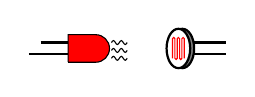
\begin{tikzpicture}[scale=0.5]
	%LED
	\draw [thick] (0,0) -- (1,0);
	\draw [thick] (0.3,0.3) -- (1,0.3);
	\draw [fill=red] (1,-0.2) -- (1,0.5) -- (1.7,0.5) arc [start angle=90,end angle=-90,radius=0.35] -- (1,-0.2);
	%Lichtstrahlen
	\draw (2.1,-0.1) sin ++(0.05,0.05) cos ++(0.05,-0.05) sin ++(0.05,-0.05) cos ++(0.05,0.05) sin ++(0.05,0.05) cos ++(0.05,-0.05) sin ++(0.05,-0.05) cos ++(0.05,0.05);
	\draw (2.1,0.1) sin ++(0.05,0.05) cos ++(0.05,-0.05) sin ++(0.05,-0.05) cos ++(0.05,0.05) sin ++(0.05,0.05) cos ++(0.05,-0.05) sin ++(0.05,-0.05) cos ++(0.05,0.05);
	\draw (2.1,0.3) sin ++(0.05,0.05) cos ++(0.05,-0.05) sin ++(0.05,-0.05) cos ++(0.05,0.05) sin ++(0.05,0.05) cos ++(0.05,-0.05) sin ++(0.05,-0.05) cos ++(0.05,0.05);
	% LDR
	\draw [thick] (4,0) -- (5,0);
	\draw [thick] (4,0.3) -- (5,0.3);
	\draw [thick,fill=gray] (3.9,0.15) ellipse [x radius=0.3,y radius=0.5];
	\draw [thick,fill=white] (3.8,0.15) ellipse [x radius=0.3,y radius=0.5];
	\draw [red] (3.65,-0.1) -- ++(0,0.5) arc [start angle=-180,end angle=-360,radius=0.03] -- ++(0,-0.5) arc [start angle=-180,end angle=0,radius=0.03] -- ++(0,0.5) arc [start angle=-180,end angle=-360,radius=0.03] -- ++(0,-0.5) arc [start angle=-180,end angle=0,radius=0.03] -- ++(0,0.5) arc [start angle=-180,end angle=-360,radius=0.03] -- ++(0,-0.5);
\end{tikzpicture}